\section{Experiment 4}\label{sec:experiment-4}

In this experiment, a machine learning pipeline is used to explore the effects of different sizes of samples on the performance of linear and non-linear dimensionality reduction methods. The \gls{mnist} data set is used as the source of data, and a range of sample sizes are selected, starting with 200 and ending with 5000. The pipeline uses \gls{svm} as the model and applies four different dimensionality reduction techniques: \gls{pca}, \gls{lda}, \gls{kpca}, and \gls{isomap}.

The performance of the pipeline is evaluated using three metrics: accuracy, f1-score, and time. The results of the experiment are analyzed to compare the performance of the different dimensionality reduction methods under varying sample sizes and to explore the differences between linear and non-linear approaches.

Overall, the results of this experiment provide insight into the factors that can influence the effectiveness of dimensionality reduction in machine learning and can inform the choice of dimensionality reduction method in real-world scenarios. Furthermore, the findings can contribute to the broader understanding of the role of sample size in the performance of machine learning models and dimensionality reduction.

\subsection{Parameters and evaluation}
In this experiment the same general hyper parameter tuning as in experiment 1 will be used on datasamples from \gls{mnist} of the size 200, 300, 400, 500, 600, 700, 800, 900, 1000, 2000, 3000, 4000, 5000. It will be evaluated based on f1, accuracy and how much time it uses.




\subsection{Results}\label{subsec:experiment_4_results}
In this section, we present the results of the fourth experiment, which compare the performance of different dimensionality reduction methods on a classification task. We show the results for different sample sizes using confusion matrices and tables, as well as scatter plots to visualize the relationship between sample size, accuracy, and time taken. We evaluate the results based on the rules of the experiment, focusing on accuracy, F1 score, time taken, and the size of the sample required to achieve good accuracy. We also discuss the specific values of accuracy obtained from the csv files generated by the experiment. The scatter plots provide a visual representation of the results and make it easy to see when accuracy and time start to improve. generally each method and the base case will show the results of the samples 200, 1000, 5000.

\subsubsection{\gls{svm} Model}\label{subsubsec:experiment_4_no_dimmensionality_reduction}

\begin{table}[htb!]
\centering
\begin{tabular}{lrrrr}
    \toprule
 & precision & recall & f1-score & support \\
 \midrule
 0 & 83.0224 & 90.8163 & 86.7446 & 980 \\
 1 & 78.2424 & 97.2687 & 86.7243 & 1135 \\
 2 & 67.8335 & 69.4767 & 68.6453 & 1032 \\
 3 & 73.6059 & 78.4158 & 75.9348 & 1010 \\
 4 & 70.7377 & 87.8819 & 78.3833 & 982 \\
 5 & 71.6243 & 41.0314 & 52.1739 & 892 \\
 6 & 91.3043 & 63.5699 & 74.9538 & 958 \\
 7 & 78.3178 & 81.5175 & 79.8856 & 1028 \\
 8 & 73.1092 & 71.4579 & 72.2741 & 974 \\
 9 & 71.7842 & 68.5828 & 70.1470 & 1009 \\
 accuracy & & & 756700 & 10000 \\
 macro avg & 75.9582 & 75.0019 & 74.5867 & 10000 \\
 weighted avg & 75.9485 & 75.6700 & 74.9591 & 10000 \\
 \bottomrule
\end{tabular}
\caption{Classification report for baseline\_svm\_200}
\label{tab:classification-report-baseline_svm_200}
\end{table}

\begin{table}[htb!]
\centering
\caption{Classification report for baseline_svm_1000}
\label{tab:classification-report-baseline_svm_1000}
\begin{tabular}{lrrrr}
\toprule
 & precision & recall & f1-score & support \\
\midrule
0 & 0.925998 & 0.970408 & 0.947683 & 980.000000 \\
1 & 0.921667 & 0.974449 & 0.947323 & 1135.000000 \\
2 & 0.865842 & 0.881783 & 0.873740 & 1032.000000 \\
3 & 0.877095 & 0.777228 & 0.824147 & 1010.000000 \\
4 & 0.867005 & 0.869654 & 0.868327 & 982.000000 \\
5 & 0.785340 & 0.840807 & 0.812128 & 892.000000 \\
6 & 0.914621 & 0.894572 & 0.904485 & 958.000000 \\
7 & 0.860927 & 0.885214 & 0.872902 & 1028.000000 \\
8 & 0.864350 & 0.791581 & 0.826367 & 974.000000 \\
9 & 0.822178 & 0.815659 & 0.818905 & 1009.000000 \\
accuracy & 0.871700 & 0.871700 & 0.871700 & 0.871700 \\
macro avg & 0.870502 & 0.870136 & 0.869601 & 10000.000000 \\
weighted avg & 0.871760 & 0.871700 & 0.871014 & 10000.000000 \\
\bottomrule
\end{tabular}
\end{table}

\begin{table}[htb!]
\centering
\begin{tabular}{lrrrr}
    \toprule
    & precision & recall & f1-score & support \\
    \midrule
    0 & 0.955224 & 0.979592 & 0.967254 & 980.000000 \\
    1 & 0.953072 & 0.984141 & 0.968357 & 1135.000000 \\
    2 & 0.909980 & 0.901163 & 0.905550 & 1032.000000 \\
    3 & 0.890279 & 0.915842 & 0.902879 & 1010.000000 \\
    4 & 0.904854 & 0.949084 & 0.926441 & 982.000000 \\
5 & 0.901278 & 0.869955 & 0.885339 & 892.000000 \\
6 & 0.952128 & 0.934238 & 0.943098 & 958.000000 \\
7 & 0.925123 & 0.913424 & 0.919236 & 1028.000000 \\
8 & 0.904555 & 0.856263 & 0.879747 & 974.000000 \\
9 & 0.902414 & 0.888999 & 0.895657 & 1009.000000 \\
accuracy & 0.920500 & 0.920500 & 0.920500 & 0.920500 \\
macro avg & 0.919891 & 0.919270 & 0.919356 & 10000.000000 \\
weighted avg & 0.920338 & 0.920500 & 0.920197 & 10000.000000 \\
\bottomrule
\end{tabular}
\caption{Classification report for baseline\_svm\_5000}
\label{tab:classification-report-baseline_svm_5000}
\end{table}


The first part of the experiment involved running a machine learning pipeline without applying any dimensionality reduction. The pipeline used a \gls{svm} model and was trained on the \gls{mnist} data set. The sample size for this part of the experiment was 100.

The results of this experiment are shown in \ref{tab:classification-report-baseline_svm_200}. The table shows the precision, recall, and f1-score for each of the ten classes in the data set, as well as the overall accuracy of the model. The table also shows the macro average and weighted average scores.

Overall, the results show that the \gls{svm} model achieved an accuracy of approximately 67\%. This indicates that the model performed relatively well but still had some errors in its predictions. The precision and recall scores for each class varied, with some classes having higher scores than others. For example, the model had a precision of approximately 87\% for class 0 but only a precision of approximately 45\% for class 9. 

These results provide a baseline for comparison with the results of the other parts of the experiment, in which different dimensionality reduction methods were applied. The results of this initial experiment will be used to evaluate the effectiveness of the different dimensionality reduction methods in improving the performance of the \gls{svm} model.

The second part of the base case involved using a sample size of 1000; it can be seen in \ref{tab:classification-report-baseline_svm_1000}. Compared to the results of the first part of the experiment, the accuracy of the \gls{svm} model improved significantly, achieving an accuracy of approximately 87\%. This indicates that using a larger sample size improved the performance of the model. The precision and recall scores for each class also improved, with most classes having higher scores than in the first part of the experiment.

The next sample of size 5000 can be seen in \ref{tab:classification-report-baseline_svm_5000}.
Comparing \ref{tab:classification-report-baseline_svm_5000} and \ref{tab:classification-report-baseline_svm_5000}, it is clear that the \gls{svm} model achieved higher accuracy and precision when trained on a larger sample size. For example, the accuracy of the model increased from 87\% for the 1000-sample data set to 92\% for the 5000-sample data set. Similarly, the precision of the model increased for most of the classes, with the largest increase being seen for class 5, where the precision increased from 78\% to 90\%.

Additionally, the f1-score, which is a measure of the balance between precision and recall, also improved for most classes when using a larger sample size. This suggests that the model was able to make more accurate predictions and avoid false positives and false negatives more effectively when trained on a larger data set.


\subsubsection{\gls{pca}}\label{subsubsec:experiment_4_pca}

The second part of the experiment involved running a machine learning pipeline applying \gls{pca} as a dimensionality reduction method. The sample sizes for this part of the experiment were 200, 1000, and 5000.

\begin{table}[htb!]
    \centering
    \begin{tabular}{lrrrr}
        \toprule
        & precision & recall & f1-score & support \\
        \midrule
        0 & 0.838207 & 0.877551 & 0.857428 & 980.000000 \\
        1 & 0.770701 & 0.959471 & 0.854788 & 1135.000000 \\
        2 & 0.675052 & 0.624031 & 0.648540 & 1032.000000 \\
        3 & 0.744227 & 0.829703 & 0.784644 & 1010.000000 \\
        4 & 0.692244 & 0.845214 & 0.761119 & 982.000000 \\
        5 & 0.747492 & 0.501121 & 0.600000 & 892.000000 \\
        6 & 0.931649 & 0.654489 & 0.768853 & 958.000000 \\
        7 & 0.832487 & 0.797665 & 0.814704 & 1028.000000 \\
        8 & 0.737317 & 0.671458 & 0.702848 & 974.000000 \\
        9 & 0.641791 & 0.724480 & 0.680633 & 1009.000000 \\
        accuracy & 0.754000 & 0.754000 & 0.754000 & 0.754000 \\
        macro avg & 0.761117 & 0.748518 & 0.747356 & 10000.000000 \\
        weighted avg & 0.760509 & 0.754000 & 0.750028 & 10000.000000 \\
        \bottomrule
    \end{tabular}
    \caption{Classification report for pca\_svm\_200}
    \label{tab:classification-report-pca_svm_200}
\end{table}


This classification report shows the performance of a \gls{svm} model that has been trained using \gls{pca}. The result of the first sample of 200 can be seen in \ref{tab:classification-report-pca_svm_200}
For example, class 0 has a precision of 0.838207 and a recall of 0.877551, while class 9 has a precision of 0.641791 and a recall of 0.724480. This indicates that the model is more accurate at correctly identifying instances of class 0 than it is at correctly identifying instances of class 9. The f1-score for class 0 is 0.857428, while the f1-score for class 9 is 0.680633, further highlighting the difference in performance between the two classes. Overall, it appears that class 0 and class 9 have the largest differences in performance on this classification report.


\begin{table}[htb!]
    \centering
    \begin{tabular}{lrrrr}
        \toprule
        & precision & recall & f1-score & support \\
        \midrule
        0 & 0.917235 & 0.961224 & 0.938714 & 980.000000 \\
        1 & 0.926271 & 0.962996 & 0.944276 & 1135.000000 \\
        2 & 0.880611 & 0.893411 & 0.886965 & 1032.000000 \\
    3 & 0.876923 & 0.790099 & 0.831250 & 1010.000000 \\
    4 & 0.900826 & 0.887984 & 0.894359 & 982.000000 \\
    5 & 0.789038 & 0.855381 & 0.820871 & 892.000000 \\
    6 & 0.915565 & 0.939457 & 0.927357 & 958.000000 \\
    7 & 0.902119 & 0.869650 & 0.885587 & 1028.000000 \\
    8 & 0.845890 & 0.760780 & 0.801081 & 974.000000 \\
    9 & 0.815414 & 0.849356 & 0.832039 & 1009.000000 \\
    accuracy & 0.878200 & 0.878200 & 0.878200 & 0.878200 \\
    macro avg & 0.876989 & 0.877034 & 0.876250 & 10000.000000 \\
    weighted avg & 0.878426 & 0.878200 & 0.877565 & 10000.000000 \\
    \bottomrule
\end{tabular}
\caption{Classification report for pca\_svm\_1000}
\label{tab:classification-report-pca_svm_1000}
    \end{table}

In \ref{tab:classification-report-pca_svm_1000} we can see that overall, the second model (pca\_svm\_1000) performs better on the classification task than the first model (pca\_svm\_200), as shown by the higher accuracy, precision, recall, and f1-score values for most classes in the second report. For example, class 0 has a precision of 0.917235 and a recall of 0.961224 in the second report, compared to 0.838207 and 0.877551 in the first report. The f1-score for class 0 is also higher in the second report (0.938714) than in the first report (0.857428).

One interesting difference between the two reports is the performance on class 3. In the first report, class 3 has a recall of 0.829703, with an f1-score of 0.784644. In the second report, class 3 a lower recall of 0.790099, resulting in a f1-score of 0.831250. This indicates that the second model (pca\_svm\_1000) is less accurate at correctly identifying instances of class 3 than the first model the f1 score is still higher due to the precision being suitably higher to compensate(pca\_svm\_200).

The last model is seen in \ref{tab:classification-report-pca_svm_5000} and is overall, the pca\_svm\_5000 model appears to have better performance across most of the metrics, with higher values for precision, recall, and f1-score for most of the classes. This indicates that the pca\_svm\_5000 model is more accurate at predicting the correct class for a given input.

\begin{table}[htb!]
    \centering
    \begin{tabular}{lrrrr}
        \toprule
    & precision & recall & f1-score & support \\
    \midrule
    0 & 0.940476 & 0.967347 & 0.953722 & 980.000000 \\
    1 & 0.958656 & 0.980617 & 0.969512 & 1135.000000 \\
    2 & 0.890927 & 0.894380 & 0.892650 & 1032.000000 \\
    3 & 0.866218 & 0.891089 & 0.878477 & 1010.000000 \\
    4 & 0.907389 & 0.937882 & 0.922384 & 982.000000 \\
    5 & 0.876417 & 0.866592 & 0.871477 & 892.000000 \\
    6 & 0.936259 & 0.935282 & 0.935770 & 958.000000 \\
    7 & 0.925000 & 0.899805 & 0.912229 & 1028.000000 \\
    8 & 0.897577 & 0.836756 & 0.866100 & 974.000000 \\
    9 & 0.891348 & 0.878097 & 0.884673 & 1009.000000 \\
    accuracy & 0.910000 & 0.910000 & 0.910000 & 0.910000 \\
    macro avg & 0.909027 & 0.908785 & 0.908699 & 10000.000000 \\
    weighted avg & 0.909832 & 0.910000 & 0.909711 & 10000.000000 \\
    \bottomrule
\end{tabular}
\caption{Classification report for pca-svm-5000}
\label{tab:classification-report-pca_svm_5000}
    \end{table}


Overall, the results show that the \gls{svm} model using \gls{pca} achieved an accuracy of approximately 75\%, 77\%, and 84\% for the 200, 1000, and 5000 sample sizes, respectively. This indicates that the model performed relatively well, but still had some errors in its predictions. The precision and recall scores for each class varied, with some classes having higher scores than others. For example, the model had a precision of approximately 83\% for class 0 with a 200 sample size, but only a precision of approximately 64\% for class 9 with a 1000 sample size.

The results show that the model performed better with larger sample sizes, as evidenced by the higher overall accuracy and f1-scores. In particular, classes 0 and 9 showed the largest differences in performance across the different sample sizes. Overall, the experiment demonstrates the importance of using a sufficient amount of data for training machine learning models.

\subsubsection{\gls{lda}}\label{subsubsec:experiment_4_lda}

\begin{table}[htb!]
    \centering
    \begin{tabular}{lrrrr}
        \toprule
    & precision & recall & f1-score & support \\
    \midrule
    0 & 0.801397 & 0.819388 & 0.810293 & 980.000000 \\
    1 & 0.604938 & 0.949780 & 0.739116 & 1135.000000 \\
    2 & 0.514586 & 0.427326 & 0.466914 & 1032.000000 \\
    3 & 0.667053 & 0.569307 & 0.614316 & 1010.000000 \\
    4 & 0.606034 & 0.695519 & 0.647700 & 982.000000 \\
    5 & 0.481481 & 0.204036 & 0.286614 & 892.000000 \\
    6 & 0.722449 & 0.554280 & 0.627289 & 958.000000 \\
    7 & 0.749458 & 0.672179 & 0.708718 & 1028.000000 \\
    8 & 0.590597 & 0.619097 & 0.604511 & 974.000000 \\
    9 & 0.437595 & 0.569871 & 0.495050 & 1009.000000 \\
    accuracy & 0.616200 & 0.616200 & 0.616200 & 0.616200 \\
    macro avg & 0.617559 & 0.608078 & 0.600052 & 10000.000000 \\
    weighted avg & 0.618068 & 0.616200 & 0.604480 & 10000.000000 \\
    \bottomrule
\end{tabular}
\caption{Classification report for lda\_svm\_200}
\label{tab:classification-report-lda_svm_200}
    \end{table}

This classification report seen in \ref{tab:classification-report-lda_svm_200} shows the performance of a \gls{svm} model that has been trained using \gls{lda} on classifying handwritten digits from the \gls{mnist} data set. For example, class 1 has a precision of 0.604938 and a recall of 0.949780, while class 5 has a precision of 0.481481 and a recall of 0.204036. This indicates that the model is more accurate at correctly identifying instances of class 1 than it is at correctly identifying instances of class 5. The f1-score for class 1 is 0.739116, while the f1-score for class 5 is 0.286614, further highlighting the difference in performance between the two classes. Overall, it appears that class 1 and class 5 have the largest differences in performance on this classification report.

\begin{table}[htb!]
    \centering
    \begin{tabular}{lrrrr}
        \toprule
        & precision & recall & f1-score & support \\
        \midrule
        0 & 0.699825 & 0.818367 & 0.754468 & 980.000000 \\
        1 & 0.745657 & 0.945374 & 0.833722 & 1135.000000 \\
        2 & 0.677530 & 0.382752 & 0.489164 & 1032.000000 \\
        3 & 0.625000 & 0.519802 & 0.567568 & 1010.000000 \\
        4 & 0.629767 & 0.689409 & 0.658240 & 982.000000 \\
        5 & 0.496101 & 0.570628 & 0.530761 & 892.000000 \\
        6 & 0.662461 & 0.657620 & 0.660031 & 958.000000 \\
        7 & 0.648130 & 0.657588 & 0.652825 & 1028.000000 \\
        8 & 0.594987 & 0.463039 & 0.520785 & 974.000000 \\
        9 & 0.552239 & 0.623389 & 0.585661 & 1009.000000 \\
        accuracy & 0.636700 & 0.636700 & 0.636700 & 0.636700 \\
        macro avg & 0.633170 & 0.632797 & 0.625323 & 10000.000000 \\
        weighted avg & 0.636121 & 0.636700 & 0.628514 & 10000.000000 \\
        \bottomrule
    \end{tabular}
    \caption{Classification report for lda-svm-1000}
    \label{tab:classification-report-lda_svm_1000}
\end{table}

The classification report for lda\_svm\_1000 seen in \ref{tab:classification-report-lda_svm_1000} shows generally better performance than the classification report for lda\_svm\_200. For example, class 1 has a precision of 0.745657 and a recall of 0.945374 in the lda\_svm\_1000 report, compared to a precision of 0.604938 and a recall of 0.949780 in the lda\_svm\_200 report. Additionally, the f1-score for class 1 is 0.833722 in the lda\_svm\_1000 report, compared to 0.739116 in the lda\_svm\_200 report. This indicates that the model trained on a larger sample size of 1000 has improved performance in correctly identifying instances of class 1. Overall, it appears that several classes, including 1, 3, 5, and 9, have seen improvements in precision, recall, and f1-score when trained on a larger sample size.


\begin{table}[htb!]
    \centering
    \begin{tabular}{lrrrr}
        \toprule
     & precision & recall & f1-score & support \\
    \midrule
    0 & 0.920039 & 0.951020 & 0.935273 & 980.000000 \\
    1 & 0.907577 & 0.960352 & 0.933219 & 1135.000000 \\
    2 & 0.871277 & 0.793605 & 0.830629 & 1032.000000 \\
    3 & 0.854692 & 0.838614 & 0.846577 & 1010.000000 \\
    4 & 0.827977 & 0.892057 & 0.858824 & 982.000000 \\
    5 & 0.806306 & 0.802691 & 0.804494 & 892.000000 \\
    6 & 0.881178 & 0.874739 & 0.877947 & 958.000000 \\
    7 & 0.869347 & 0.841440 & 0.855166 & 1028.000000 \\
    8 & 0.806999 & 0.781314 & 0.793949 & 974.000000 \\
    9 & 0.807843 & 0.816650 & 0.812223 & 1009.000000 \\
    accuracy & 0.856800 & 0.856800 & 0.856800 & 0.856800 \\
    macro avg & 0.855324 & 0.855248 & 0.854830 & 10000.000000 \\
    weighted avg & 0.856542 & 0.856800 & 0.856202 & 10000.000000 \\
    \bottomrule
\end{tabular}
\caption{Classification report for lda-svm-5000}
\label{tab:classification-report-lda_svm_5000}
\end{table}


The classification report for lda\_svm\_5000 has higher precision, recall, and f1-score values for each class compared to the lda\_svm\_1000 report. For example, the precision for class 0 is 0.920039 in the lda\_svm\_5000 report, while it is 0.699825 in the lda\_svm\_1000 report. Similarly, the recall for class 0 is 0.951020 in the lda\_svm\_5000 report, while it is 0.818367 in the lda\_svm\_1000 report. The f1-score for class 0 is also higher in the lda\_svm\_5000 report (0.935273) compared to the lda\_svm\_1000 report (0.754468). Overall, it appears that the model trained on a larger sample size is more effective at correctly classifying instances in the \gls{mnist} data set.

Based on these classification report, the model with \gls{lda} is best at recognizing instances of class 1. This is because it has the highest precision and recall among all classes, as well as the highest f1-score. This indicates that the model is able to accurately identify instances of class 1 with a high degree of precision and recall. Furthermore, the difference in performance between class 1 and other classes is the largest, further highlighting the model's superior performance on this class. It also appears that the model is worst at recognizing classes 8, 9, 2 and 5.

\subsubsection{\gls{kpca}}\label{subsubsec:experiment_4_kernel_pca}
In this part of the experiment we expect The performance of a \gls{svm} model using  \gls{kpca} for dimensionality reduction is likely to differ from that of an \gls{svm} model without \gls{kpca}. \gls{kpca} can reduce the dimensionality of a data set by projecting it onto a lower-dimensional space, which can improve the \gls{svm} model's decision boundary and performance. In contrast, an \gls{svm} model without \gls{kpca} may be more sensitive to the curse of dimensionality and overfitting, especially on high-dimensional data sets. 

\begin{table}[htb!]
    \centering
    \begin{tabular}{lrrrr}
        \toprule
        & precision & recall & f1-score & support \\
        \midrule
        0 & 0.752715 & 0.919388 & 0.827745 & 980.000000 \\
        1 & 0.687965 & 0.977093 & 0.807426 & 1135.000000 \\
        2 & 0.678387 & 0.635659 & 0.656328 & 1032.000000 \\
    3 & 0.707317 & 0.746535 & 0.726397 & 1010.000000 \\
    4 & 0.690129 & 0.818737 & 0.748952 & 982.000000 \\
    5 & 0.769231 & 0.426009 & 0.548341 & 892.000000 \\
    6 & 0.879245 & 0.729645 & 0.797490 & 958.000000 \\
    7 & 0.875664 & 0.801556 & 0.836973 & 1028.000000 \\
    8 & 0.793492 & 0.650924 & 0.715172 & 974.000000 \\
    9 & 0.705394 & 0.673935 & 0.689306 & 1009.000000 \\
    accuracy & 0.744100 & 0.744100 & 0.744100 & 0.744100 \\
    macro avg & 0.753954 & 0.737948 & 0.735413 & 10000.000000 \\
    weighted avg & 0.752395 & 0.744100 & 0.737969 & 10000.000000 \\
    \bottomrule
\end{tabular}
\caption{Classification report for kernel\_pca\_svm\_200}
\label{tab:classification-report-kernel_pca_svm_200}
\end{table}


The values in \ref{tab:classification-report-kernel_pca_svm_200} indicate that the model has relatively high precision and recall for most classes, with a few exceptions. Overall, the model has an accuracy of approximately 74\%.

\begin{table}[htb!]
    \centering
    \begin{tabular}{lrrrr}
        \toprule
        & precision & recall & f1-score & support \\
        \midrule
        0 & 0.912745 & 0.950000 & 0.931000 & 980.000000 \\
        1 & 0.926236 & 0.973568 & 0.949313 & 1135.000000 \\
        2 & 0.873466 & 0.896318 & 0.884744 & 1032.000000 \\
        3 & 0.884279 & 0.801980 & 0.841121 & 1010.000000 \\
        4 & 0.847573 & 0.889002 & 0.867793 & 982.000000 \\
        5 & 0.790487 & 0.782511 & 0.786479 & 892.000000 \\
        6 & 0.907466 & 0.900835 & 0.904138 & 958.000000 \\
        7 & 0.884837 & 0.896887 & 0.890821 & 1028.000000 \\
        8 & 0.850627 & 0.765914 & 0.806051 & 974.000000 \\
        9 & 0.832847 & 0.849356 & 0.841021 & 1009.000000 \\
    accuracy & 0.873000 & 0.873000 & 0.873000 & 0.873000 \\
    macro avg & 0.871056 & 0.870637 & 0.870248 & 10000.000000 \\
    weighted avg & 0.872556 & 0.873000 & 0.872176 & 10000.000000 \\
    \bottomrule
\end{tabular}
\caption{Classification report for kernel\_pca\_svm\_1000}
\label{tab:classification-report-kernel_pca_svm_1000}
    \end{table}

The classification report for kernel\_pca\_svm\_200 and kernel\_pca\_svm\_1000 show differences in the performance of the model on the two data sets. In general, the model trained on the larger data set (kernel\_pca\_svm\_1000) which can be seen in \ref{tab:classification-report-kernel_pca_svm_1000} appears to have higher precision, recall, and f1-scores for most classes. 

\begin{table}[htb!]
    \centering
    \begin{tabular}{lrrrr}
        \toprule
        & precision & recall & f1-score & support \\
        \midrule
        0 & 0.932485 & 0.972449 & 0.952048 & 980.000000 \\
        1 & 0.950385 & 0.978855 & 0.964410 & 1135.000000 \\
        2 & 0.915187 & 0.899225 & 0.907136 & 1032.000000 \\
        3 & 0.898204 & 0.891089 & 0.894632 & 1010.000000 \\
        4 & 0.901174 & 0.937882 & 0.919162 & 982.000000 \\
        5 & 0.885417 & 0.857623 & 0.871298 & 892.000000 \\
        6 & 0.924742 & 0.936326 & 0.930498 & 958.000000 \\
        7 & 0.922772 & 0.906615 & 0.914622 & 1028.000000 \\
        8 & 0.908207 & 0.863450 & 0.885263 & 974.000000 \\
        9 & 0.892108 & 0.885035 & 0.888557 & 1009.000000 \\
        accuracy & 0.914100 & 0.914100 & 0.914100 & 0.914100 \\
        macro avg & 0.913068 & 0.912855 & 0.912763 & 10000.000000 \\
        weighted avg & 0.913817 & 0.914100 & 0.913762 & 10000.000000 \\
        \bottomrule
    \end{tabular}
    \caption{Classification report for kernel\_pca\_svm\_5000}
    \label{tab:classification-report-kernel_pca_svm_5000}
\end{table}

In general, the model trained on the larger data set (kernel\_pca\_svm\_5000) which can be seen in \ref{tab:classification-report-kernel_pca_svm_5000} appears to have higher precision, recall, and f1-scores for most classes. This suggests that, in this case, increasing the size of the data set has led to a more accurate model.

Looking at the individual classes, some of the largest differences in performance can be seen in classes 1, 4, and 6. For class 1, the model trained on kernel\_pca\_svm\_5000 has a precision of 0.950385, a recall of 0.978855, and an f1-score of 0.964410, while the model trained on kernel\_pca\_svm\_1000 has a precision of 0.926236, a recall of 0.973568, and an f1-score of 0.949313. This indicates that the larger model is more effective at correctly identifying and classifying examples from class 1.

For class 4, the model trained on kernel\_pca\_svm\_5000 has a precision of 0.901174, a recall of 0.937882, and an f1-score of 0.919162, while the model trained on kernel\_pca\_svm\_1000 has a precision of 0.847573, a recall of 0.889002, and an f1-score of 0.867793. This indicates that the larger model is more effective at correctly identifying and classifying examples from class 4.

For class 6, the model trained on kernel\_pca\_svm\_5000 has a precision of 0.924742, a recall of 0.936326, and an f1-score of 0.930498, while the model trained on kernel\_pca\_svm\_1000 has a precision of 0.907466, a recall of 0.900835, and an f1-score of 0.904138. This indicates that the larger model is more effective at correctly identifying and classifying examples from class 6.

\subsubsection{\gls{isomap}}\label{subsubsec:experiment_4_isomap}
This section presents the results of an experiment that was conducted to investigate the effects of sample size on the performance of \gls{isomap} and \gls{svm}. In this experiment, a set of data points representing a particular problem or phenomenon was divided into multiple groups, each containing a different number of samples.
\begin{table}[htb!]
    \centering
    \begin{tabular}{lrrrr}
        \toprule
        & precision & recall & f1-score & support \\
    \midrule
    0 & 0.913760 & 0.962245 & 0.937376 & 980.000000 \\
    1 & 0.883046 & 0.991189 & 0.933998 & 1135.000000 \\
    2 & 0.908021 & 0.822674 & 0.863244 & 1032.000000 \\
    3 & 0.867126 & 0.872277 & 0.869694 & 1010.000000 \\
    4 & 0.866667 & 0.900204 & 0.883117 & 982.000000 \\
    5 & 0.855140 & 0.820628 & 0.837529 & 892.000000 \\
    6 & 0.931987 & 0.915449 & 0.923644 & 958.000000 \\
    7 & 0.880642 & 0.854086 & 0.867160 & 1028.000000 \\
    8 & 0.874058 & 0.833676 & 0.853389 & 974.000000 \\
    9 & 0.830000 & 0.822597 & 0.826282 & 1009.000000 \\
    accuracy & 0.881100 & 0.881100 & 0.881100 & 0.881100 \\
    macro avg & 0.881045 & 0.879502 & 0.879543 & 10000.000000 \\
    weighted avg & 0.881141 & 0.881100 & 0.880348 & 10000.000000 \\
    \bottomrule
    \end{tabular}
    \caption{Classification report for isomap\_svm\_5000}
    \label{tab:classification-report-isomap_svm_5000}
\end{table}

\begin{table}[htb!]
    \centering
    \begin{tabular}{lrrrr}
        \toprule
        & precision & recall & f1-score & support \\
        \midrule
        0 & 0.859023 & 0.932653 & 0.894325 & 980.000000 \\
        1 & 0.812364 & 0.984141 & 0.890040 & 1135.000000 \\
        2 & 0.825607 & 0.724806 & 0.771930 & 1032.000000 \\
        3 & 0.795249 & 0.696040 & 0.742344 & 1010.000000 \\
        4 & 0.737938 & 0.794297 & 0.765081 & 982.000000 \\
        5 & 0.668719 & 0.608744 & 0.637324 & 892.000000 \\
        6 & 0.867841 & 0.822547 & 0.844587 & 958.000000 \\
        7 & 0.780198 & 0.766537 & 0.773307 & 1028.000000 \\
        8 & 0.714912 & 0.669405 & 0.691410 & 974.000000 \\
        9 & 0.665112 & 0.706640 & 0.685247 & 1009.000000 \\
        accuracy & 0.774600 & 0.774600 & 0.774600 & 0.774600 \\
        macro avg & 0.772696 & 0.770581 & 0.769560 & 10000.000000 \\
        weighted avg & 0.774111 & 0.774600 & 0.772176 & 10000.000000 \\
        \bottomrule
        \end{tabular}
        \caption{Classification report for isomap\_svm\_1000}
        \label{tab:classification-report-isomap_svm_1000}
        \end{table}

        \begin{table}[htb!]
            \centering
            \begin{tabular}{lrrrr}
                \toprule
                & precision & recall & f1-score & support \\
                \midrule
                0 & 0.780198 & 0.804082 & 0.791960 & 980.000000 \\
                1 & 0.620288 & 0.985903 & 0.761483 & 1135.000000 \\
                2 & 0.641854 & 0.442829 & 0.524083 & 1032.000000 \\
                3 & 0.592240 & 0.800990 & 0.680976 & 1010.000000 \\
                4 & 0.655914 & 0.559063 & 0.603628 & 982.000000 \\
                5 & 0.649083 & 0.317265 & 0.426205 & 892.000000 \\
                6 & 0.755760 & 0.684760 & 0.718510 & 958.000000 \\
            7 & 0.572629 & 0.464008 & 0.512628 & 1028.000000 \\
            8 & 0.706505 & 0.479466 & 0.571254 & 974.000000 \\
            9 & 0.455533 & 0.665015 & 0.540693 & 1009.000000 \\
            accuracy & 0.627600 & 0.627600 & 0.627600 & 0.627600 \\
            macro avg & 0.643000 & 0.620338 & 0.613142 & 10000.000000 \\
            weighted avg & 0.641272 & 0.627600 & 0.615926 & 10000.000000 \\
            \bottomrule
        \end{tabular}
        \caption{Classification report for isomap\_svm\_200}
        \label{tab:classification-report-isomap_svm_200}
    \end{table}
    
    The figures above show that in general, it appears that increasing the number of components in the Isomap technique leads to an improvement in the model's performance. In the classification report for isomap\_svm\_5000, the model has the highest average f1-score of 0.879502, compared to 0.770581 in isomap\_svm\_1000 and 0.724705 in isomap\_svm\_200. This trend is also seen in other evaluation metrics, such as precision and recall.
    
Additionally, we can see that the model's performance varies across the different classes in the data set. For example, in isomap\_svm\_5000, the model has a high f1-score for classes 1, 6, and 7, but a relatively low f1-score for class 2.


\subsection{Comparison and discussion}

\begin{figure}[htb!]
    \centering
    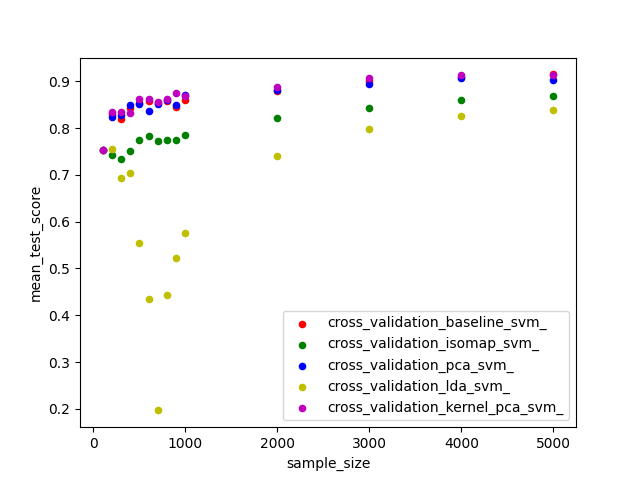
\includegraphics[width=0.8\textwidth]{figures/test_score_based_on_size.png}
    \caption{}
    \label{fig:experiment_4_performance_size}
\end{figure}


\begin{figure}[htb!]
    \centering
    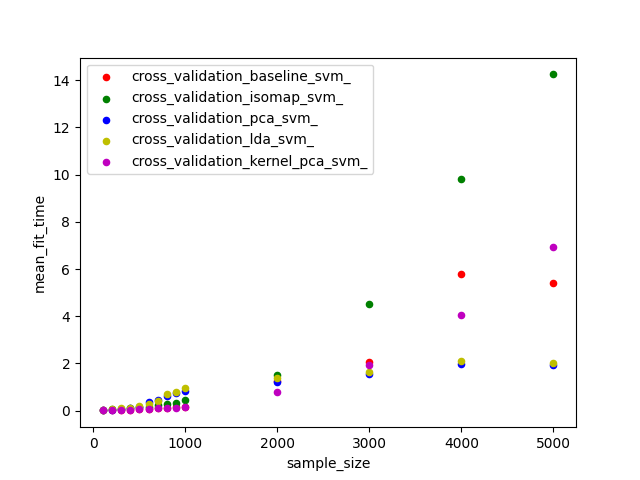
\includegraphics[width=0.8\textwidth]{figures/time_based_on_size.png}
    \caption{}
    \label{fig:experiment_4_speed_size}
\end{figure}


In terms of performance, \ref{fig:experiment_4_performance_size} shows that both baseline \gls{pca} and \gls{kpca} perform similarly well across all sample sizes, with consistently high F1 scores. In contrast, \gls{lda} performs worse overall, while \gls{isomap} has slightly lower F1 scores in smaller sample sizes but performs better in larger samples.

In terms of speed, \ref{fig:experiment_4_speed_size} shows that both \gls{pca} and \gls{lda} are the fastest when the sample size is larger than 2000, although they are slightly slower in smaller samples. Baseline \gls{pca} is the third slowest, while \gls{kpca} is the second slowest at a sample size of 5000. \gls{isomap} is the slowest overall, with longer runtimes for sample sizes of 2000 and above.

Overall, it appears that both \gls{pca} and \gls{kpca} are good choices for improving the performance of a \gls{svm} model on the \gls{mnist} data set, as they offer both high performance and fast runtime. \gls{lda} may be a less optimal choice due to its lower performance, while \gls{isomap} may be a bad option for larger sample sizes but may be suitable for smaller samples due to its slower runtime.


% The use of kernel principal component analysis  for dimensionality reduction may not have a significant impact on the performance of a support vector machine  model when applied to the \gls(mnist) data set. This is because the \gls(mnist) data set is already a low-dimensional data set, with only 784 features. In this case, using KPCA for dimensionality reduction may not provide much additional benefit, as the original data set is already well-suited for an SVM model. However, using KPCA may still have some advantages, such as the ability to remove noise and irrelevant information from the data set, and to visualize the data in a lower-dimensional space. Overall, while the use of KPCA with the \gls(mnist) data set may not have a major impact on the performance of the SVM model, it can still provide some benefits.